% Options for packages loaded elsewhere
\PassOptionsToPackage{unicode}{hyperref}
\PassOptionsToPackage{hyphens}{url}
%
\documentclass[
]{article}
\usepackage{lmodern}
\usepackage{amssymb,amsmath}
\usepackage{ifxetex,ifluatex}
\ifnum 0\ifxetex 1\fi\ifluatex 1\fi=0 % if pdftex
  \usepackage[T1]{fontenc}
  \usepackage[utf8]{inputenc}
  \usepackage{textcomp} % provide euro and other symbols
\else % if luatex or xetex
  \usepackage{unicode-math}
  \defaultfontfeatures{Scale=MatchLowercase}
  \defaultfontfeatures[\rmfamily]{Ligatures=TeX,Scale=1}
\fi
% Use upquote if available, for straight quotes in verbatim environments
\IfFileExists{upquote.sty}{\usepackage{upquote}}{}
\IfFileExists{microtype.sty}{% use microtype if available
  \usepackage[]{microtype}
  \UseMicrotypeSet[protrusion]{basicmath} % disable protrusion for tt fonts
}{}
\makeatletter
\@ifundefined{KOMAClassName}{% if non-KOMA class
  \IfFileExists{parskip.sty}{%
    \usepackage{parskip}
  }{% else
    \setlength{\parindent}{0pt}
    \setlength{\parskip}{6pt plus 2pt minus 1pt}}
}{% if KOMA class
  \KOMAoptions{parskip=half}}
\makeatother
\usepackage{xcolor}
\IfFileExists{xurl.sty}{\usepackage{xurl}}{} % add URL line breaks if available
\IfFileExists{bookmark.sty}{\usepackage{bookmark}}{\usepackage{hyperref}}
\hypersetup{
  hidelinks,
  pdfcreator={LaTeX via pandoc}}
\urlstyle{same} % disable monospaced font for URLs
\usepackage{color}
\usepackage{fancyvrb}
\newcommand{\VerbBar}{|}
\newcommand{\VERB}{\Verb[commandchars=\\\{\}]}
\DefineVerbatimEnvironment{Highlighting}{Verbatim}{commandchars=\\\{\}}
% Add ',fontsize=\small' for more characters per line
\newenvironment{Shaded}{}{}
\newcommand{\AlertTok}[1]{\textcolor[rgb]{1.00,0.00,0.00}{\textbf{#1}}}
\newcommand{\AnnotationTok}[1]{\textcolor[rgb]{0.38,0.63,0.69}{\textbf{\textit{#1}}}}
\newcommand{\AttributeTok}[1]{\textcolor[rgb]{0.49,0.56,0.16}{#1}}
\newcommand{\BaseNTok}[1]{\textcolor[rgb]{0.25,0.63,0.44}{#1}}
\newcommand{\BuiltInTok}[1]{#1}
\newcommand{\CharTok}[1]{\textcolor[rgb]{0.25,0.44,0.63}{#1}}
\newcommand{\CommentTok}[1]{\textcolor[rgb]{0.38,0.63,0.69}{\textit{#1}}}
\newcommand{\CommentVarTok}[1]{\textcolor[rgb]{0.38,0.63,0.69}{\textbf{\textit{#1}}}}
\newcommand{\ConstantTok}[1]{\textcolor[rgb]{0.53,0.00,0.00}{#1}}
\newcommand{\ControlFlowTok}[1]{\textcolor[rgb]{0.00,0.44,0.13}{\textbf{#1}}}
\newcommand{\DataTypeTok}[1]{\textcolor[rgb]{0.56,0.13,0.00}{#1}}
\newcommand{\DecValTok}[1]{\textcolor[rgb]{0.25,0.63,0.44}{#1}}
\newcommand{\DocumentationTok}[1]{\textcolor[rgb]{0.73,0.13,0.13}{\textit{#1}}}
\newcommand{\ErrorTok}[1]{\textcolor[rgb]{1.00,0.00,0.00}{\textbf{#1}}}
\newcommand{\ExtensionTok}[1]{#1}
\newcommand{\FloatTok}[1]{\textcolor[rgb]{0.25,0.63,0.44}{#1}}
\newcommand{\FunctionTok}[1]{\textcolor[rgb]{0.02,0.16,0.49}{#1}}
\newcommand{\ImportTok}[1]{#1}
\newcommand{\InformationTok}[1]{\textcolor[rgb]{0.38,0.63,0.69}{\textbf{\textit{#1}}}}
\newcommand{\KeywordTok}[1]{\textcolor[rgb]{0.00,0.44,0.13}{\textbf{#1}}}
\newcommand{\NormalTok}[1]{#1}
\newcommand{\OperatorTok}[1]{\textcolor[rgb]{0.40,0.40,0.40}{#1}}
\newcommand{\OtherTok}[1]{\textcolor[rgb]{0.00,0.44,0.13}{#1}}
\newcommand{\PreprocessorTok}[1]{\textcolor[rgb]{0.74,0.48,0.00}{#1}}
\newcommand{\RegionMarkerTok}[1]{#1}
\newcommand{\SpecialCharTok}[1]{\textcolor[rgb]{0.25,0.44,0.63}{#1}}
\newcommand{\SpecialStringTok}[1]{\textcolor[rgb]{0.73,0.40,0.53}{#1}}
\newcommand{\StringTok}[1]{\textcolor[rgb]{0.25,0.44,0.63}{#1}}
\newcommand{\VariableTok}[1]{\textcolor[rgb]{0.10,0.09,0.49}{#1}}
\newcommand{\VerbatimStringTok}[1]{\textcolor[rgb]{0.25,0.44,0.63}{#1}}
\newcommand{\WarningTok}[1]{\textcolor[rgb]{0.38,0.63,0.69}{\textbf{\textit{#1}}}}
\usepackage{graphicx,grffile}
\makeatletter
\def\maxwidth{\ifdim\Gin@nat@width>\linewidth\linewidth\else\Gin@nat@width\fi}
\def\maxheight{\ifdim\Gin@nat@height>\textheight\textheight\else\Gin@nat@height\fi}
\makeatother
% Scale images if necessary, so that they will not overflow the page
% margins by default, and it is still possible to overwrite the defaults
% using explicit options in \includegraphics[width, height, ...]{}
\setkeys{Gin}{width=\maxwidth,height=\maxheight,keepaspectratio}
% Set default figure placement to htbp
\makeatletter
\def\fps@figure{htbp}
\makeatother
\setlength{\emergencystretch}{3em} % prevent overfull lines
\providecommand{\tightlist}{%
  \setlength{\itemsep}{0pt}\setlength{\parskip}{0pt}}
\setcounter{secnumdepth}{-\maxdimen} % remove section numbering

\date{}

\begin{document}

\begin{titlepage}
\vfill
\begin{center}

\includegraphics[width=2cm]{../Images/index.jpeg}
\\[1cm]
\begin{LARGE}
\uppercase{College of Engineering}
\\[0.3cm]
\uppercase{Trivandrum}
\end{LARGE}
\\[1.5cm]
\uppercase{Computer science and engineering}
\\[0.2cm]
\uppercase{Application software development lab}
\\[0.5cm]
{\Large CSE 333}
\\[1cm]
{\Large\uppercase{Application software development\\[0.1cm]lab exam report}}
\\[0.5cm]
\uppercase{Certified bonafide record of work done by}
\\[0.5cm]
\uppercase{Rwithik Manoj}
\\[0.4cm]
\textsc{University Reg. No: TVE17CS054}
\\[0.4cm]
\textsc{Roll No: 53}
\\[0.4cm]
\textsc{Class: S5 CSE}
\end{center}
\vfill
\textsc{Staff In-charge:}\\[0.4cm]
VIPIN VASU A.V, REMYA KRISHNAN\\[0.4cm]
\textsc{Department of Computer Science and Engineering}
\end{titlepage}

\begin{enumerate}
\def\labelenumi{\arabic{enumi}.}
\tightlist
\item
  Create and populate shown tables. Check the following constraints:

  \begin{enumerate}
  \def\labelenumii{\arabic{enumii}.}
  \tightlist
  \item
    Song\_ID should be of the format ``S00\_\_''
  \item
    Album\_ID should be of the format ``AL00\_\_'',
  \item
    Album\_ID should be of the format ``AL00\_\_'',
  \item
    Artist\_ID should be of the format ``AR00\_\_''.
  \end{enumerate}
\end{enumerate}

\begin{Shaded}
\begin{Highlighting}[]
\KeywordTok{create} \KeywordTok{table}\NormalTok{ song(}
\NormalTok{   songid }\DataTypeTok{varchar}\NormalTok{(}\DecValTok{10}\NormalTok{) }\KeywordTok{check}\NormalTok{(songid }\KeywordTok{like} \StringTok{\textquotesingle{}S00\_\_\textquotesingle{}}\NormalTok{),}
\NormalTok{   songname }\DataTypeTok{varchar}\NormalTok{(}\DecValTok{25}\NormalTok{),}
\NormalTok{   albumid }\DataTypeTok{varchar}\NormalTok{(}\DecValTok{10}\NormalTok{) }\KeywordTok{check}\NormalTok{(albumid }\KeywordTok{like} \StringTok{\textquotesingle{}AL00\_\_\textquotesingle{}}\NormalTok{),}
\NormalTok{   genre }\DataTypeTok{varchar}\NormalTok{(}\DecValTok{10}\NormalTok{),}
\NormalTok{   views }\DataTypeTok{integer}\NormalTok{);}

\KeywordTok{INSERT} \KeywordTok{INTO}\NormalTok{ song }\KeywordTok{VALUES}\NormalTok{(}\StringTok{\textquotesingle{}S0001\textquotesingle{}}\NormalTok{, }\StringTok{\textquotesingle{}Panic and Sentiment\textquotesingle{}}\NormalTok{, }\StringTok{\textquotesingle{}AL0004\textquotesingle{}}\NormalTok{, }\StringTok{\textquotesingle{}Pop\textquotesingle{}}\NormalTok{, }\DecValTok{450}\NormalTok{);}
\KeywordTok{INSERT} \KeywordTok{INTO}\NormalTok{ song }\KeywordTok{VALUES}\NormalTok{(}\StringTok{\textquotesingle{}S0002\textquotesingle{}}\NormalTok{, }\StringTok{\textquotesingle{}Addicted to Dignity\textquotesingle{}}\NormalTok{, }\StringTok{\textquotesingle{}AL0001\textquotesingle{}}\NormalTok{, }\StringTok{\textquotesingle{}Rap\textquotesingle{}}\NormalTok{, }\DecValTok{600}\NormalTok{);}
\KeywordTok{INSERT} \KeywordTok{INTO}\NormalTok{ song }\KeywordTok{VALUES}\NormalTok{(}\StringTok{\textquotesingle{}S0003\textquotesingle{}}\NormalTok{, }\StringTok{\textquotesingle{}Expressed\textquotesingle{}}\NormalTok{, }\StringTok{\textquotesingle{}AL0002\textquotesingle{}}\NormalTok{, }\StringTok{\textquotesingle{}Pop\textquotesingle{}}\NormalTok{, }\DecValTok{500}\NormalTok{);}
\KeywordTok{INSERT} \KeywordTok{INTO}\NormalTok{ song }\KeywordTok{VALUES}\NormalTok{(}\StringTok{\textquotesingle{}S0004\textquotesingle{}}\NormalTok{, }\StringTok{\textquotesingle{}Promise to Science\textquotesingle{}}\NormalTok{, }\StringTok{\textquotesingle{}AL0005\textquotesingle{}}\NormalTok{, }\StringTok{\textquotesingle{}Rock\textquotesingle{}}\NormalTok{, }\DecValTok{920}\NormalTok{);}
\KeywordTok{INSERT} \KeywordTok{INTO}\NormalTok{ song }\KeywordTok{VALUES}\NormalTok{(}\StringTok{\textquotesingle{}S0005\textquotesingle{}}\NormalTok{, }\StringTok{\textquotesingle{}Comfortable Illusion\textquotesingle{}}\NormalTok{, }\StringTok{\textquotesingle{}AL0003\textquotesingle{}}\NormalTok{, }\StringTok{\textquotesingle{}Rock\textquotesingle{}}\NormalTok{, }\DecValTok{760}\NormalTok{);}
\KeywordTok{INSERT} \KeywordTok{INTO}\NormalTok{ song }\KeywordTok{VALUES}\NormalTok{(}\StringTok{\textquotesingle{}S0006\textquotesingle{}}\NormalTok{, }\StringTok{\textquotesingle{}Handicapped Bomber\textquotesingle{}}\NormalTok{, }\StringTok{\textquotesingle{}AL0002\textquotesingle{}}\NormalTok{, }\StringTok{\textquotesingle{}Rap\textquotesingle{}}\NormalTok{, }\DecValTok{1000}\NormalTok{);}
\KeywordTok{INSERT} \KeywordTok{INTO}\NormalTok{ song }\KeywordTok{VALUES}\NormalTok{(}\StringTok{\textquotesingle{}S0007\textquotesingle{}}\NormalTok{, }\StringTok{\textquotesingle{}Default Agenda\textquotesingle{}}\NormalTok{, }\StringTok{\textquotesingle{}AL0004\textquotesingle{}}\NormalTok{, }\StringTok{\textquotesingle{}Jazz\textquotesingle{}}\NormalTok{, }\DecValTok{260}\NormalTok{);}
\KeywordTok{INSERT} \KeywordTok{INTO}\NormalTok{ song }\KeywordTok{VALUES}\NormalTok{(}\StringTok{\textquotesingle{}S0008\textquotesingle{}}\NormalTok{, }\StringTok{\textquotesingle{}Tropical River\textquotesingle{}}\NormalTok{, }\StringTok{\textquotesingle{}AL0002\textquotesingle{}}\NormalTok{, }\StringTok{\textquotesingle{}Pop\textquotesingle{}}\NormalTok{, }\DecValTok{420}\NormalTok{);}

\KeywordTok{create} \KeywordTok{table}\NormalTok{ album(}
\NormalTok{   albumid }\DataTypeTok{varchar}\NormalTok{(}\DecValTok{10}\NormalTok{) }\KeywordTok{check}\NormalTok{(albumid }\KeywordTok{like} \StringTok{\textquotesingle{}AL00\_\_\textquotesingle{}}\NormalTok{),}
\NormalTok{   albumname }\DataTypeTok{varchar}\NormalTok{(}\DecValTok{25}\NormalTok{),}
\NormalTok{   artistid }\DataTypeTok{varchar}\NormalTok{(}\DecValTok{10}\NormalTok{) }\KeywordTok{check}\NormalTok{(artistid }\KeywordTok{like} \StringTok{\textquotesingle{}AR00\_\_\textquotesingle{}}\NormalTok{),}
\NormalTok{   releasedate }\DataTypeTok{date}\NormalTok{,}
\NormalTok{   sales }\DataTypeTok{integer}\NormalTok{);}

\KeywordTok{INSERT} \KeywordTok{INTO}\NormalTok{ album }\KeywordTok{VALUES}\NormalTok{(}\StringTok{\textquotesingle{}AL0001\textquotesingle{}}\NormalTok{, }\StringTok{\textquotesingle{}Jurisdiction\textquotesingle{}}\NormalTok{, }\StringTok{\textquotesingle{}AR0004\textquotesingle{}}\NormalTok{, }\StringTok{\textquotesingle{}16{-}03{-}2004\textquotesingle{}}\NormalTok{, }\DecValTok{570}\NormalTok{);}
\KeywordTok{INSERT} \KeywordTok{INTO}\NormalTok{ album }\KeywordTok{VALUES}\NormalTok{(}\StringTok{\textquotesingle{}AL0002\textquotesingle{}}\NormalTok{, }\StringTok{\textquotesingle{}Limitless\textquotesingle{}}\NormalTok{, }\StringTok{\textquotesingle{}AR0003\textquotesingle{}}\NormalTok{, }\StringTok{\textquotesingle{}24{-}05{-}2007\textquotesingle{}}\NormalTok{, }\DecValTok{650}\NormalTok{);}
\KeywordTok{INSERT} \KeywordTok{INTO}\NormalTok{ album }\KeywordTok{VALUES}\NormalTok{(}\StringTok{\textquotesingle{}AL0003\textquotesingle{}}\NormalTok{, }\StringTok{\textquotesingle{}69 cents\textquotesingle{}}\NormalTok{, }\StringTok{\textquotesingle{}AR0001\textquotesingle{}}\NormalTok{, }\StringTok{\textquotesingle{}6{-}09{-}2005\textquotesingle{}}\NormalTok{, }\DecValTok{400}\NormalTok{);}
\KeywordTok{INSERT} \KeywordTok{INTO}\NormalTok{ album }\KeywordTok{VALUES}\NormalTok{(}\StringTok{\textquotesingle{}AL0004\textquotesingle{}}\NormalTok{, }\StringTok{\textquotesingle{}Confession\textquotesingle{}}\NormalTok{, }\StringTok{\textquotesingle{}AR0002\textquotesingle{}}\NormalTok{, }\StringTok{\textquotesingle{}28{-}11{-}2012\textquotesingle{}}\NormalTok{, }\DecValTok{120}\NormalTok{);}
\KeywordTok{INSERT} \KeywordTok{INTO}\NormalTok{ album }\KeywordTok{VALUES}\NormalTok{(}\StringTok{\textquotesingle{}AL0005\textquotesingle{}}\NormalTok{, }\StringTok{\textquotesingle{}Hero\textquotesingle{}}\NormalTok{, }\StringTok{\textquotesingle{}AR0004\textquotesingle{}}\NormalTok{, }\StringTok{\textquotesingle{}7{-}07{-}2002\textquotesingle{}}\NormalTok{, }\DecValTok{900}\NormalTok{);}

\KeywordTok{create} \KeywordTok{table}\NormalTok{ artist(}
\NormalTok{   artistid }\DataTypeTok{varchar}\NormalTok{(}\DecValTok{10}\NormalTok{) }\KeywordTok{check}\NormalTok{(artistid }\KeywordTok{like} \StringTok{\textquotesingle{}AR00\_\_\textquotesingle{}}\NormalTok{),}
\NormalTok{   artistname }\DataTypeTok{varchar}\NormalTok{(}\DecValTok{25}\NormalTok{),}
\NormalTok{   country }\DataTypeTok{varchar}\NormalTok{(}\DecValTok{20}\NormalTok{));}

\KeywordTok{INSERT} \KeywordTok{INTO}\NormalTok{ artist }\KeywordTok{VALUES}\NormalTok{(}\StringTok{\textquotesingle{}AR0001\textquotesingle{}}\NormalTok{, }\StringTok{\textquotesingle{}Natalia Finch\textquotesingle{}}\NormalTok{, }\StringTok{\textquotesingle{}France\textquotesingle{}}\NormalTok{);}
\KeywordTok{INSERT} \KeywordTok{INTO}\NormalTok{ artist }\KeywordTok{VALUES}\NormalTok{(}\StringTok{\textquotesingle{}AR0002\textquotesingle{}}\NormalTok{, }\StringTok{\textquotesingle{}Suman Yu\textquotesingle{}}\NormalTok{, }\StringTok{\textquotesingle{}India\textquotesingle{}}\NormalTok{);}
\KeywordTok{INSERT} \KeywordTok{INTO}\NormalTok{ artist }\KeywordTok{VALUES}\NormalTok{(}\StringTok{\textquotesingle{}AR0003\textquotesingle{}}\NormalTok{, }\StringTok{\textquotesingle{}Hill Will\textquotesingle{}}\NormalTok{, }\StringTok{\textquotesingle{}USA\textquotesingle{}}\NormalTok{);}
\KeywordTok{INSERT} \KeywordTok{INTO}\NormalTok{ artist }\KeywordTok{VALUES}\NormalTok{(}\StringTok{\textquotesingle{}AR0004\textquotesingle{}}\NormalTok{, }\StringTok{\textquotesingle{}Sham E\textquotesingle{}}\NormalTok{, }\StringTok{\textquotesingle{}France\textquotesingle{}}\NormalTok{);}

\KeywordTok{create} \KeywordTok{table}\NormalTok{ grammy (}
   \DataTypeTok{year} \DataTypeTok{integer}\NormalTok{, songid }\DataTypeTok{varchar}\NormalTok{(}\DecValTok{10}\NormalTok{));}

\KeywordTok{INSERT} \KeywordTok{INTO}\NormalTok{ grammy }\KeywordTok{VALUES}\NormalTok{(}\DecValTok{2003}\NormalTok{, }\StringTok{\textquotesingle{}S0004\textquotesingle{}}\NormalTok{);}
\KeywordTok{INSERT} \KeywordTok{INTO}\NormalTok{ grammy }\KeywordTok{VALUES}\NormalTok{(}\DecValTok{2007}\NormalTok{, }\StringTok{\textquotesingle{}S0006\textquotesingle{}}\NormalTok{);}
\KeywordTok{INSERT} \KeywordTok{INTO}\NormalTok{ grammy }\KeywordTok{VALUES}\NormalTok{(}\DecValTok{2009}\NormalTok{, }\StringTok{\textquotesingle{}S0003\textquotesingle{}}\NormalTok{);}
\KeywordTok{INSERT} \KeywordTok{INTO}\NormalTok{ grammy }\KeywordTok{VALUES}\NormalTok{(}\DecValTok{2004}\NormalTok{, }\StringTok{\textquotesingle{}S0002\textquotesingle{}}\NormalTok{);}
\KeywordTok{INSERT} \KeywordTok{INTO}\NormalTok{ grammy }\KeywordTok{VALUES}\NormalTok{(}\DecValTok{2012}\NormalTok{, }\StringTok{\textquotesingle{}S0007\textquotesingle{}}\NormalTok{);}
\end{Highlighting}
\end{Shaded}

\begin{enumerate}
\def\labelenumi{\arabic{enumi}.}
\setcounter{enumi}{1}
\tightlist
\item
  List all the songs by Sham E in the year 2002.
\end{enumerate}

\begin{Shaded}
\begin{Highlighting}[]
\KeywordTok{select}\NormalTok{ songname }\KeywordTok{from}\NormalTok{ song s, artist a, album b }
   \KeywordTok{where}\NormalTok{ a.artistname }\OperatorTok{=} \StringTok{\textquotesingle{}Sham E\textquotesingle{}} \KeywordTok{AND}\NormalTok{ a.artistid }\OperatorTok{=}\NormalTok{ b.artistid }
      \KeywordTok{and}\NormalTok{ s.albumid}\OperatorTok{=}\NormalTok{b.albumid }\KeywordTok{and}\NormalTok{ b.releasedate }\OperatorTok{<} \StringTok{\textquotesingle{}2003{-}01{-}01\textquotesingle{}} 
      \KeywordTok{and}\NormalTok{ b.releasedate }\OperatorTok{>} \StringTok{\textquotesingle{}2001{-}12{-}31\textquotesingle{}}\NormalTok{;}
\end{Highlighting}
\end{Shaded}

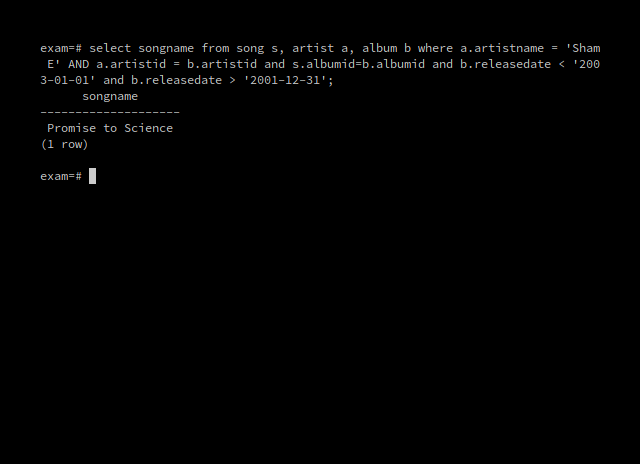
\includegraphics{../Images/Exam_Report/1.png}

\begin{enumerate}
\def\labelenumi{\arabic{enumi}.}
\setcounter{enumi}{2}
\tightlist
\item
  List all songs in the same album as Expressed.
\end{enumerate}

\begin{Shaded}
\begin{Highlighting}[]
\KeywordTok{select}\NormalTok{ songname }\KeywordTok{from}\NormalTok{ song s }\KeywordTok{where} 
\NormalTok{   s.albumid }\KeywordTok{in} 
\NormalTok{   (}\KeywordTok{select}\NormalTok{ albumid }\KeywordTok{from}\NormalTok{ song }\KeywordTok{where}\NormalTok{ songname }\OperatorTok{=} \StringTok{\textquotesingle{}Expressed\textquotesingle{}}\NormalTok{);}
\end{Highlighting}
\end{Shaded}

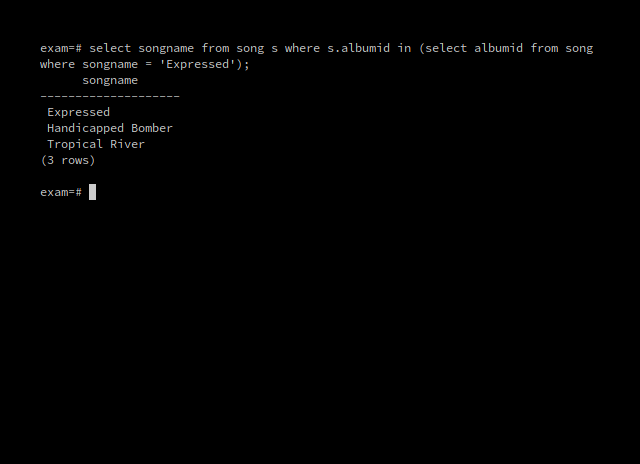
\includegraphics{../Images/Exam_Report/2.png}

\begin{enumerate}
\def\labelenumi{\arabic{enumi}.}
\setcounter{enumi}{3}
\tightlist
\item
  Display the name and total number of views of all albums with sales
  more than 500.
\end{enumerate}

\begin{Shaded}
\begin{Highlighting}[]
\KeywordTok{select}\NormalTok{ albumname, }\FunctionTok{sum}\NormalTok{(views) }\KeywordTok{from}\NormalTok{ song, album }
   \KeywordTok{where}\NormalTok{ sales }\OperatorTok{>} \DecValTok{500} \KeywordTok{and}\NormalTok{ song.albumid}\OperatorTok{=}\NormalTok{album.albumid }
   \KeywordTok{group} \KeywordTok{by}\NormalTok{ albumname;}
\end{Highlighting}
\end{Shaded}

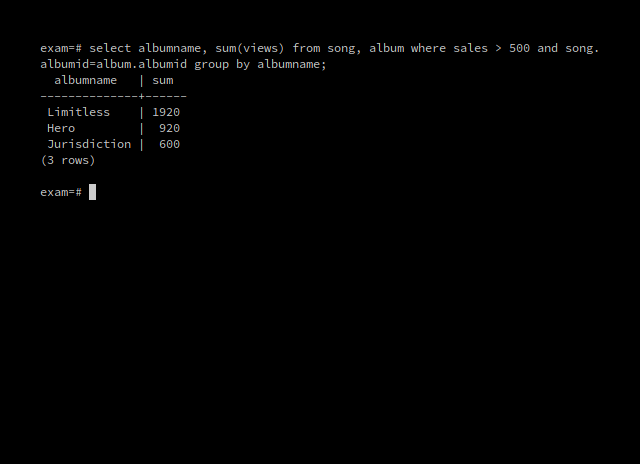
\includegraphics{../Images/Exam_Report/3.png}

\begin{enumerate}
\def\labelenumi{\arabic{enumi}.}
\setcounter{enumi}{4}
\tightlist
\item
  Display the number of songs that did not win a Grammy in each album.
\end{enumerate}

\begin{Shaded}
\begin{Highlighting}[]
\KeywordTok{select}\NormalTok{ b.albumid, }\FunctionTok{count}\NormalTok{(}\OperatorTok{*}\NormalTok{) }\KeywordTok{from}\NormalTok{ album b, song s }
   \KeywordTok{where}\NormalTok{ s.albumid }\OperatorTok{=}\NormalTok{ b.albumid }\KeywordTok{and}\NormalTok{ songid }\KeywordTok{not} \KeywordTok{in} 
\NormalTok{      (}\KeywordTok{select}\NormalTok{ songid }\KeywordTok{from}\NormalTok{ grammy) }\KeywordTok{group} \KeywordTok{by}\NormalTok{ b.albumid;}
\end{Highlighting}
\end{Shaded}

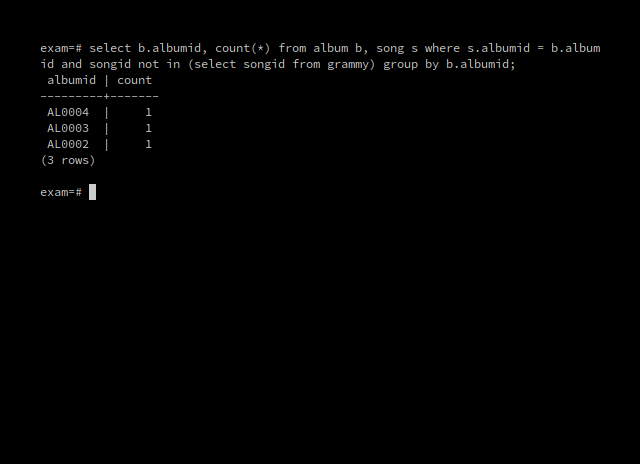
\includegraphics{../Images/Exam_Report/4.png}

\begin{enumerate}
\def\labelenumi{\arabic{enumi}.}
\setcounter{enumi}{5}
\tightlist
\item
  Create a Trigger such that whenever a new song is added, if it has
  more than 750 views, it wins a Grammy in that year itself.
\end{enumerate}

\begin{Shaded}
\begin{Highlighting}[]
\KeywordTok{create} \KeywordTok{or} \KeywordTok{replace} \KeywordTok{function}\NormalTok{ check\_grammy()}
\NormalTok{returns }\KeywordTok{trigger} \KeywordTok{as}\NormalTok{ $$}
\KeywordTok{declare}
\DataTypeTok{year} \DataTypeTok{integer} \OperatorTok{:=} \DecValTok{2019}\NormalTok{;}
\ControlFlowTok{begin}
\ControlFlowTok{if} \KeywordTok{new}\NormalTok{.views }\OperatorTok{>} \DecValTok{750} \ControlFlowTok{then}
\KeywordTok{insert} \KeywordTok{into}\NormalTok{ grammy }\KeywordTok{values}\NormalTok{(}\DataTypeTok{year}\NormalTok{, }\KeywordTok{new}\NormalTok{.songid);}
\ControlFlowTok{end} \ControlFlowTok{if}\NormalTok{;}
\KeywordTok{return} \KeywordTok{new}\NormalTok{;}
\ControlFlowTok{end}\NormalTok{;}
\NormalTok{$$ language plpgsql;}

\KeywordTok{create} \KeywordTok{trigger}\NormalTok{ grammy\_give }
   \KeywordTok{before} \KeywordTok{insert} \KeywordTok{on}\NormalTok{ song }
   \ControlFlowTok{for} \KeywordTok{each} \KeywordTok{row} 
   \KeywordTok{execute} \KeywordTok{procedure}\NormalTok{ check\_grammy();}
\end{Highlighting}
\end{Shaded}

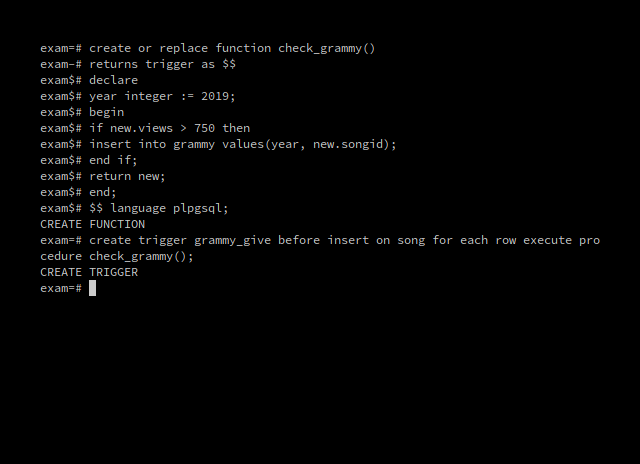
\includegraphics{../Images/Exam_Report/5.png}

\begin{enumerate}
\def\labelenumi{\arabic{enumi}.}
\setcounter{enumi}{6}
\tightlist
\item
  Create a view ``Golden Winners'' which contains the name of the
  song,album and artists which won the Grammy on the year they released.
\end{enumerate}

\begin{Shaded}
\begin{Highlighting}[]
\KeywordTok{create} \KeywordTok{view}\NormalTok{ golden\_winners }\KeywordTok{as} 
   \KeywordTok{select} \DataTypeTok{year}\NormalTok{, songname, albumname, artistname }
      \KeywordTok{from}\NormalTok{ grammy g, album b, artist a, song s }
      \KeywordTok{where} \DataTypeTok{date}\NormalTok{(}\FunctionTok{concat}\NormalTok{(}\DataTypeTok{year}\NormalTok{, }\StringTok{\textquotesingle{}{-}01{-}01\textquotesingle{}}\NormalTok{)) }\OperatorTok{<}\NormalTok{ b.releasedate }
         \KeywordTok{and} \DataTypeTok{date}\NormalTok{(}\FunctionTok{concat}\NormalTok{(}\DataTypeTok{year}\NormalTok{, }\StringTok{\textquotesingle{}{-}12{-}31\textquotesingle{}}\NormalTok{)) }\OperatorTok{>}\NormalTok{ b.releasedate }
         \KeywordTok{and}\NormalTok{ s.songid}\OperatorTok{=}\NormalTok{g.songid }\KeywordTok{and}\NormalTok{ b.albumid}\OperatorTok{=}\NormalTok{s.albumid }
         \KeywordTok{and}\NormalTok{ a.artistid}\OperatorTok{=}\NormalTok{b.artistid;}
\end{Highlighting}
\end{Shaded}

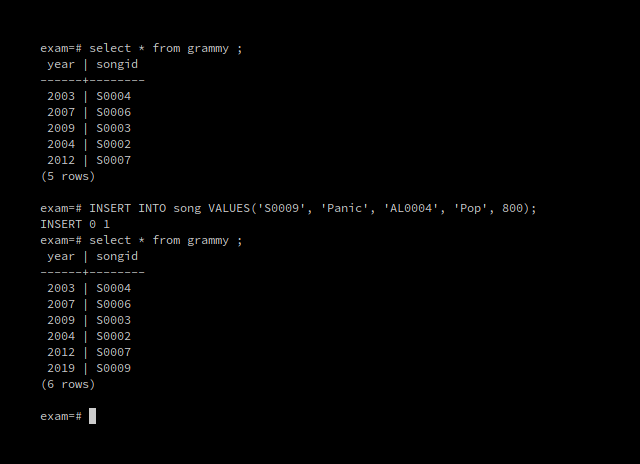
\includegraphics{../Images/Exam_Report/6.png}

\begin{enumerate}
\def\labelenumi{\arabic{enumi}.}
\setcounter{enumi}{7}
\tightlist
\item
  Decrease the sales by 10\% for all albums released before 2009.
  Perform the operation using cursor.
\end{enumerate}

\begin{Shaded}
\begin{Highlighting}[]
\KeywordTok{create} \KeywordTok{or} \KeywordTok{replace} \KeywordTok{function}\NormalTok{ dec\_sales()}
\NormalTok{returns }\DataTypeTok{integer} \KeywordTok{as}\NormalTok{ $$}
\KeywordTok{declare}
\NormalTok{cur }\KeywordTok{cursor} \ControlFlowTok{for} \KeywordTok{select} \OperatorTok{*} \KeywordTok{from}\NormalTok{ album;}
\NormalTok{rec }\DataTypeTok{record}\NormalTok{;}
\ControlFlowTok{begin}
\KeywordTok{open}\NormalTok{ cur;}
\ControlFlowTok{loop}
\NormalTok{fetch cur }\KeywordTok{into}\NormalTok{ rec;}
\NormalTok{exit }\ControlFlowTok{when} \KeywordTok{not}\NormalTok{ found;}
\ControlFlowTok{if}\NormalTok{ rec.releasedate }\OperatorTok{<} \StringTok{\textquotesingle{}2009{-}01{-}01\textquotesingle{}} \ControlFlowTok{then}
\KeywordTok{update}\NormalTok{ album }\KeywordTok{set} 
\NormalTok{   sales }\OperatorTok{=} \FloatTok{0.9} \OperatorTok{*}\NormalTok{ sales }
   \KeywordTok{where} \KeywordTok{current} \KeywordTok{of}\NormalTok{ cur;}
\ControlFlowTok{end} \ControlFlowTok{if}\NormalTok{;}
\ControlFlowTok{end} \ControlFlowTok{loop}\NormalTok{;}
\KeywordTok{return} \KeywordTok{null}\NormalTok{;}
\ControlFlowTok{end}\NormalTok{;}
\NormalTok{$$}
\NormalTok{language plpgsql;}
\end{Highlighting}
\end{Shaded}

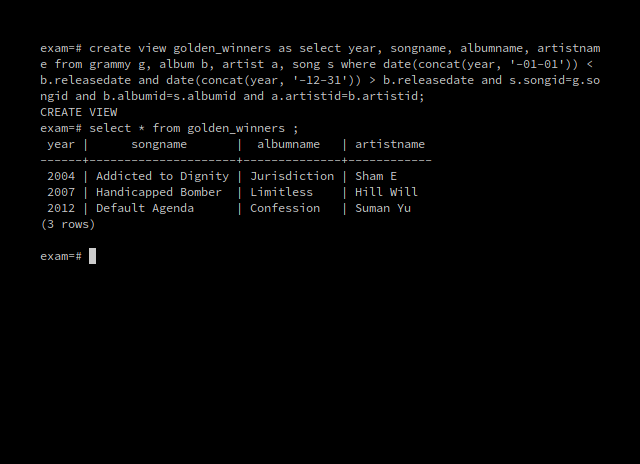
\includegraphics{../Images/Exam_Report/7.png}

\begin{enumerate}
\def\labelenumi{\arabic{enumi}.}
\setcounter{enumi}{8}
\tightlist
\item
  You are given a table, BST, containing two columns: N and P, where N
  represents the value of a node in a Binary Tree, and P is the parent
  of N. Write a query to find the node type of Binary Tree ordered by
  the value of the node. Output one of the following for each node:

  \begin{itemize}
  \tightlist
  \item
    Root: If node is the root node.
  \item
    Leaf: If node is leaf node.
  \item
    Inner: If node is neither root nor leaf node
  \end{itemize}
\end{enumerate}

\begin{Shaded}
\begin{Highlighting}[]
\KeywordTok{create} \KeywordTok{table}\NormalTok{ bst(}
\NormalTok{n }\DataTypeTok{integer}\NormalTok{,}
\NormalTok{p }\DataTypeTok{integer}\NormalTok{);}

\KeywordTok{INSERT} \KeywordTok{INTO}\NormalTok{ bst }\KeywordTok{VALUES}\NormalTok{(}\DecValTok{1}\NormalTok{, }\DecValTok{2}\NormalTok{);}
\KeywordTok{INSERT} \KeywordTok{INTO}\NormalTok{ bst }\KeywordTok{VALUES}\NormalTok{(}\DecValTok{3}\NormalTok{, }\DecValTok{2}\NormalTok{);}
\KeywordTok{INSERT} \KeywordTok{INTO}\NormalTok{ bst }\KeywordTok{VALUES}\NormalTok{(}\DecValTok{6}\NormalTok{, }\DecValTok{8}\NormalTok{);}
\KeywordTok{INSERT} \KeywordTok{INTO}\NormalTok{ bst }\KeywordTok{VALUES}\NormalTok{(}\DecValTok{9}\NormalTok{, }\DecValTok{8}\NormalTok{);}
\KeywordTok{INSERT} \KeywordTok{INTO}\NormalTok{ bst }\KeywordTok{VALUES}\NormalTok{(}\DecValTok{2}\NormalTok{, }\DecValTok{5}\NormalTok{);}
\KeywordTok{INSERT} \KeywordTok{INTO}\NormalTok{ bst }\KeywordTok{VALUES}\NormalTok{(}\DecValTok{8}\NormalTok{, }\DecValTok{5}\NormalTok{);}
\KeywordTok{INSERT} \KeywordTok{INTO}\NormalTok{ bst(n) }\KeywordTok{VALUES}\NormalTok{(}\DecValTok{5}\NormalTok{);}

\KeywordTok{select}\NormalTok{ n, }\ControlFlowTok{case}
\ControlFlowTok{when}\NormalTok{ p }\KeywordTok{is} \KeywordTok{null} \ControlFlowTok{then} \StringTok{\textquotesingle{}Root\textquotesingle{}}
\ControlFlowTok{when} \KeywordTok{exists}\NormalTok{ (}\KeywordTok{select} \OperatorTok{*} \KeywordTok{from}\NormalTok{ bst b2 }\KeywordTok{where}\NormalTok{ b2.p}\OperatorTok{=}\NormalTok{b1.n) }\ControlFlowTok{then} \StringTok{\textquotesingle{}Inner\textquotesingle{}}
\ControlFlowTok{else} \StringTok{\textquotesingle{}Leaf\textquotesingle{}}
\ControlFlowTok{end}
\KeywordTok{from}\NormalTok{ bst b1 }\KeywordTok{order} \KeywordTok{by}\NormalTok{ n;}
\end{Highlighting}
\end{Shaded}

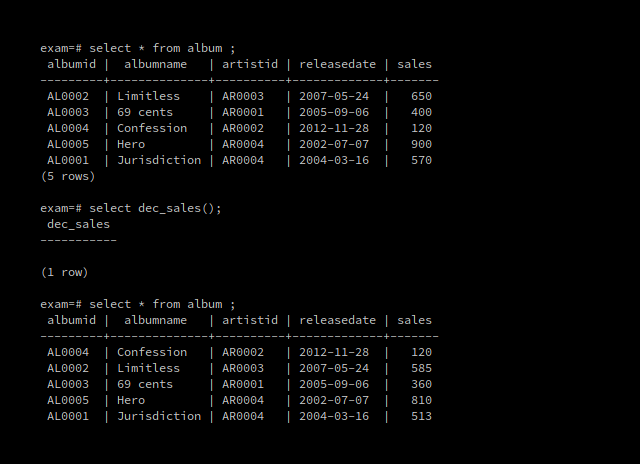
\includegraphics{../Images/Exam_Report/8.png}

\begin{enumerate}
\def\labelenumi{\arabic{enumi}.}
\setcounter{enumi}{9}
\tightlist
\item
  For the above database, multiply the sales value of all albums which
  have received grammy award with the number of grammys received and
  update the sales column.
\end{enumerate}

\begin{Shaded}
\begin{Highlighting}[]
\KeywordTok{create} \KeywordTok{or} \KeywordTok{replace} \KeywordTok{function}\NormalTok{ upd()}
\NormalTok{returns }\DataTypeTok{integer} \KeywordTok{as}\NormalTok{ $$}
\KeywordTok{declare}
\NormalTok{cur }\KeywordTok{cursor} \ControlFlowTok{for} \KeywordTok{select} \OperatorTok{*} \KeywordTok{from}\NormalTok{ album;}
\NormalTok{cnt }\DataTypeTok{integer}
\NormalTok{rec }\DataTypeTok{record}\NormalTok{;}
\ControlFlowTok{begin}
    \KeywordTok{open}\NormalTok{ cur;}
    \ControlFlowTok{loop}
\NormalTok{    fetch cur }\KeywordTok{into}\NormalTok{ rec;}
\NormalTok{    exit }\ControlFlowTok{when} \KeywordTok{not}\NormalTok{ found;}
    \KeywordTok{select} \KeywordTok{into}\NormalTok{ cnt }\KeywordTok{from}\NormalTok{ album b, song s, grammy g}
        \KeywordTok{where}\NormalTok{ b.albumid}\OperatorTok{=}\NormalTok{s.albumid }\KeywordTok{and}\NormalTok{ g.songid}\OperatorTok{=}\NormalTok{s.songid;}
    \ControlFlowTok{if}\NormalTok{ cnt }\OperatorTok{>} \DecValTok{0} \ControlFlowTok{then}
        \KeywordTok{update}\NormalTok{ album }\KeywordTok{set}\NormalTok{ sales }\OperatorTok{=}\NormalTok{ sales }\OperatorTok{*}\NormalTok{ cnt;}
    \ControlFlowTok{end} \ControlFlowTok{if}\NormalTok{;}
    \ControlFlowTok{end} \ControlFlowTok{loop}\NormalTok{;}
\KeywordTok{close}\NormalTok{ cur;}
\KeywordTok{return} \KeywordTok{null}\NormalTok{;}
\ControlFlowTok{end}\NormalTok{;}
\NormalTok{$$ language plpgsql;}
\end{Highlighting}
\end{Shaded}

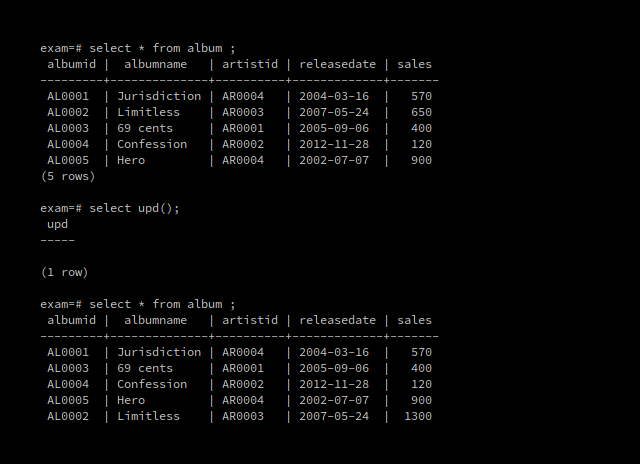
\includegraphics{../Images/Exam_Report/10.png}

\begin{enumerate}
\def\labelenumi{\arabic{enumi}.}
\setcounter{enumi}{10}
\tightlist
\item
  Write a function to find the first n Fibonacci numbers which are not
  prime and store them into a table.
\end{enumerate}

\begin{Shaded}
\begin{Highlighting}[]
\KeywordTok{create} \KeywordTok{or} \KeywordTok{replace} \KeywordTok{function}\NormalTok{ prime(n }\DataTypeTok{integer}\NormalTok{)}
\NormalTok{returns }\DataTypeTok{integer} \KeywordTok{as}
\NormalTok{$$}
\KeywordTok{declare}
\NormalTok{    i }\DataTypeTok{integer} \OperatorTok{:=} \DecValTok{1}\NormalTok{;}
\NormalTok{    j }\DataTypeTok{integer} \OperatorTok{:=} \DecValTok{1}\NormalTok{;}
\NormalTok{    k }\DataTypeTok{integer}\NormalTok{;}
\NormalTok{    c }\DataTypeTok{integer} \OperatorTok{:=} \DecValTok{0}\NormalTok{;}
\NormalTok{    flag }\DataTypeTok{integer} \OperatorTok{:=} \DecValTok{0}\NormalTok{;}
\ControlFlowTok{begin}
\NormalTok{    raise notice }\StringTok{\textquotesingle{}\%\textquotesingle{}}\NormalTok{, i;}
\NormalTok{    raise notice }\StringTok{\textquotesingle{}\%\textquotesingle{}}\NormalTok{, j;}
    \ControlFlowTok{while}\NormalTok{ c }\OperatorTok{<}\NormalTok{ n }\ControlFlowTok{loop}
        \KeywordTok{select}\NormalTok{ i}\OperatorTok{+}\NormalTok{j, i }\KeywordTok{into}\NormalTok{ i, j;}
        \ControlFlowTok{for}\NormalTok{ p }\KeywordTok{in} \DecValTok{2}\OperatorTok{..}\NormalTok{i}\OperatorTok{/}\DecValTok{2} \ControlFlowTok{loop}
            \ControlFlowTok{if}\NormalTok{ n\%p}\OperatorTok{=}\DecValTok{0} \ControlFlowTok{then}
\NormalTok{                flag }\OperatorTok{=} \DecValTok{1}\NormalTok{;}
            \ControlFlowTok{end} \ControlFlowTok{if}\NormalTok{;}
        \ControlFlowTok{end} \ControlFlowTok{loop}\NormalTok{;}
        \ControlFlowTok{if}\NormalTok{ flag}\OperatorTok{=}\DecValTok{0} \ControlFlowTok{then}
\NormalTok{            raise notice }\StringTok{\textquotesingle{}\%\textquotesingle{}}\NormalTok{, i;}
\NormalTok{            c }\OperatorTok{:=}\NormalTok{ c}\OperatorTok{+}\DecValTok{1}\NormalTok{;}
\NormalTok{            flag }\OperatorTok{:=} \DecValTok{0}\NormalTok{;}
        \ControlFlowTok{end} \ControlFlowTok{if}\NormalTok{;}
    \ControlFlowTok{end} \ControlFlowTok{loop}\NormalTok{;}
\ControlFlowTok{end}\NormalTok{;}
\NormalTok{$$}
\NormalTok{language plpgsql;}
\end{Highlighting}
\end{Shaded}

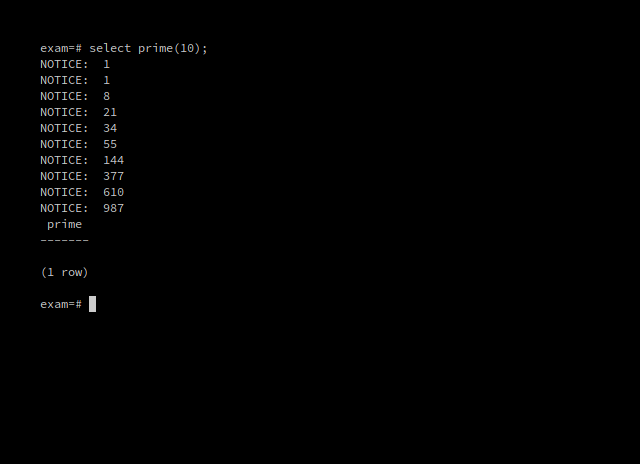
\includegraphics{../Images/Exam_Report/11.png}

\end{document}
